% This is samplepaper.tex, a sample chapter demonstrating the
% LLNCS macro package for Springer Computer Science proceedings;
% Version 2.20 of 2017/10/04
%
\documentclass[runningheads]{llncs}
%
\usepackage{graphicx}
\usepackage{comment}
\usepackage{indentfirst}
% Used for displaying a sample figure. If possible, figure files should
% be included in EPS format.
%
% If you use the hyperref package, please uncomment the following line
% to display URLs in blue roman font according to Springer's eBook style:
% \renewcommand\UrlFont{\color{blue}\rmfamily}

\begin{document}
%
\title{ECE219 Project2 Clustering}
%
%\titlerunning{Abbreviated paper title}
% If the paper title is too long for the running head, you can set
% an abbreviated paper title here
%
\author{Zhilai~Shen, Yufei~Hu, Zheang~Huai, and Tianyi~Liu
}
%
% First names are abbreviated in the running head.
% If there are more than two authors, 'et al.' is used.
%
\institute{UCLA}
%
\maketitle              % typeset the header of the contribution
%
%
%
%
\begin{comment}
\section{First Section}
\subsection{A Subsection Sample}
Please note that the first paragraph of a section or subsection is
not indented. The first paragraph that follows a table, figure,
equation etc. does not need an indent, either.

Subsequent paragraphs, however, are indented.

\subsubsection{Sample Heading (Third Level)} Only two levels of
headings should be numbered. Lower level headings remain unnumbered;
they are formatted as run-in headings.

\paragraph{Sample Heading (Fourth Level)}
The contribution should contain no more than four levels of
headings. Table~\ref{tab1} gives a summary of all heading levels.

\begin{table}
\caption{Table captions should be placed above the
tables.}\label{tab1}
\begin{tabular}{|l|l|l|}
\hline
Heading level &  Example & Font size and style\\
\hline
Title (centered) &  {\Large\bfseries Lecture Notes} & 14 point, bold\\
1st-level heading &  {\large\bfseries 1 Introduction} & 12 point, bold\\
2nd-level heading & {\bfseries 2.1 Printing Area} & 10 point, bold\\
3rd-level heading & {\bfseries Run-in Heading in Bold.} Text follows & 10 point, bold\\
4th-level heading & {\itshape Lowest Level Heading.} Text follows & 10 point, italic\\
\hline
\end{tabular}
\end{table}


\noindent Displayed equations are centered and set on a separate
line.
\begin{equation}
x + y = z
\end{equation}
Please try to avoid rasterized images for line-art diagrams and
schemas. Whenever possible, use vector graphics instead (see
Fig.~\ref{fig1}).

\begin{figure}
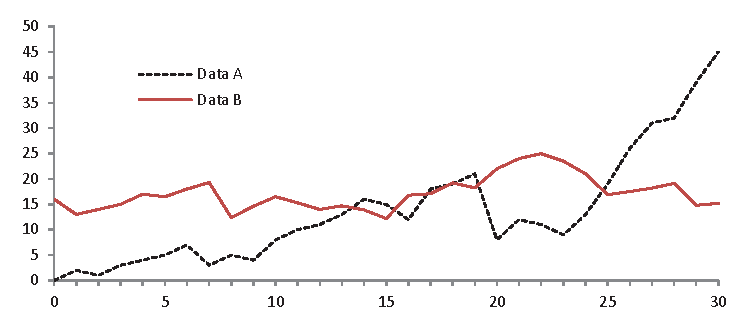
\includegraphics[width=\textwidth]{Figure/fig1.eps}
\caption{A figure caption is always placed below the illustration.
Please note that short captions are centered, while long ones are
justified by the macro package automatically.} \label{fig1}
\end{figure}

\begin{theorem}
This is a sample theorem. The run-in heading is set in bold, while
the following text appears in italics. Definitions, lemmas,
propositions, and corollaries are styled the same way.
\end{theorem}
%
% the environments 'definition', 'lemma', 'proposition', 'corollary',
% 'remark', and 'example' are defined in the LLNCS documentclass as well.
%
\begin{proof}
Proofs, examples, and remarks have the initial word in italics,
while the following text appears in normal font.
\end{proof}
For citations of references, we prefer the use of square brackets
and consecutive numbers. Citations using labels or the author/year
convention are also acceptable. The following bibliography provides
a sample reference list with entries for journal
articles~\cite{ref_article1}, an LNCS chapter~\cite{ref_lncs1}, a
book~\cite{ref_book1}, proceedings without editors~\cite{ref_proc1},
and a homepage~\cite{ref_url1}. Multiple citations are grouped
\cite{ref_article1,ref_lncs1,ref_book1},
\cite{ref_article1,ref_book1,ref_proc1,ref_url1}.
%
% ---- Bibliography ----
%
% BibTeX users should specify bibliography style 'splncs04'.
% References will then be sorted and formatted in the correct style.
%
% \bibliographystyle{splncs04}
% \bibliography{mybibliography}
%

\end{comment}

\section{Building the TF-IDF Matrix}

\textbf{Question 1:}

The dimensions of the TF-IDF matrix is: (7882, 27768).

\section{Apply K-means Clustering}

\subsection{Contingency Table}

\textbf{Question 2:}

The contingency table of the clustering result is:
\begin{center}
[[   4 3899]

 [1718 2261]]
\end{center}

As we can see, the result of K-means clustering using the TF-IDF data without dimensionality reduction is not that bad. Most points of one class can be recognized as in one cluster. But many points of the other class can't be clustered correctly.

\subsection{Measures}

\textbf{Question 3:}
The 5 measures for the K-means clustering results is shown in Table \ref{tab:q3}.

\begin{table}[h]
\center
\caption{5 measures for the K-means clustering results}
\scalebox{0.9}{
\begin{tabular}{c|c}
\hline
Homogeneity & 0.2536 \\\hline
Completeness & 0.3348 \\\hline
V-measure & 0.2886 \\\hline
Adjusted Rand Index & 0.1808 \\\hline
Adjusted mutual info score & 0.2535\\\hline
\end{tabular}}
\label{tab:q3}
\end{table}

As can be seen from the table, the scores of 5 measures are not very high, which means that the result of clustering is not very good. And we can see some reasons from question2: many points of one class are recognized as in another cluster.

\section{Dimensionality Reduction}

\subsection{Principle Components}

\textbf{Question 4:}

A plot of what ratio of the variance of the original data is retained after the dimensionality reduction is shown in Figure \ref{fig:Q4}. It's pretty obvious that this curve increases monotonically.

\begin{figure}
\centering
\scalebox{0.4}{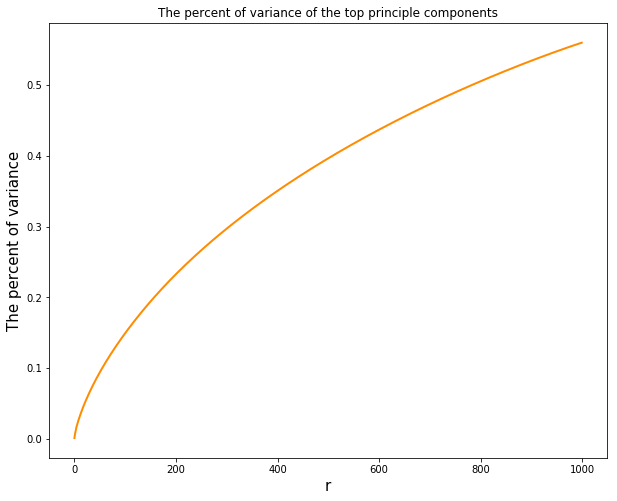
\includegraphics{Figure/Q4.png}}
\caption{The percent of variance of the top principle components} \label{fig:Q4}
\end{figure}


\subsection{PCA and NMF}

\textbf{Question 5:}

This time, we try several $r$ values for SVD and NMF respectively and their measure scores are shown in Figure \ref{fig:Q5_1}and \ref{fig:Q5_2}. When it comes to the problem of choosing the best $r$, we need to decide which measure scores we care the most. Overall speaking, homogeneity and completeness didn't measure the result very well since they only show part of the properties of the result. Therefore we choose the other three methods to decide which parameter is the best. We can see from the plot result that the best $r$ for both SVD and NMF is $2$.

\bigbreak

\begin{figure}
\centering
\scalebox{0.4}{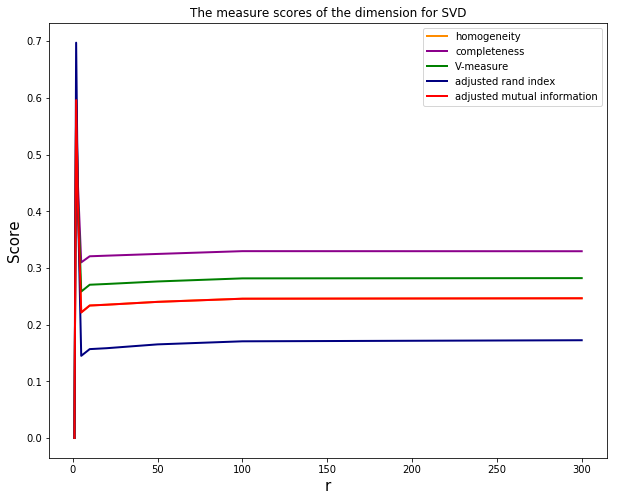
\includegraphics{Figure/Q5_1.png}}
\caption{5 measure scores for different $r$ value of SVD} \label{fig:Q5_1}
\end{figure}

\begin{figure}
\centering
\scalebox{0.4}{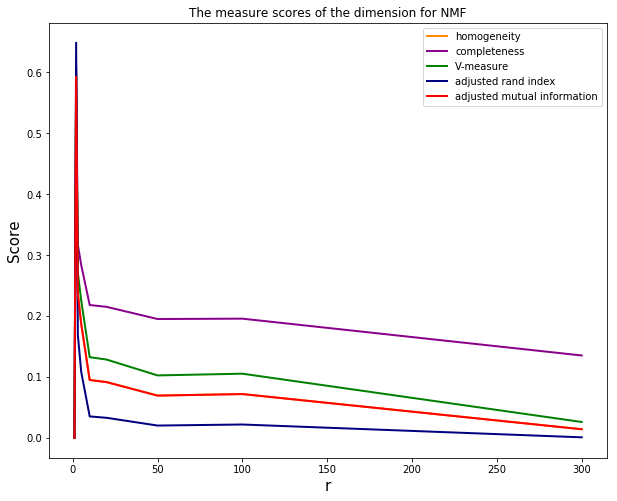
\includegraphics{Figure/Q5_2.png}}
\caption{5 measure scores for different $r$ value of NMF} \label{fig:Q5_2}
\end{figure}



\textbf{Question 6:}

What we can also see from the plot is that the curve is non-monotonic. This can be explained as when the dimension of the data is pretty high the Euclidean distance metric becomes useless since the distances between data points tends to be almost the same in the pretty sparse high dimensional space. Also as the number of dimensions grows, the relative euclidean distance between a point in a set and its closest neighbour, and between that point and its furthest neighbour, changes in some non-obvious ways. Therefore we need a best parameter $r$ which is not too small and not too big.

\section{Optimization}

\subsection{Visualization}

\textbf{Question 7:}

In this problem, we visualize the performance of clustering data with best clustering parameters derived from the previous questions. Dimension reduction are conducted using SVD and NMF respectively. The visualization can be seen below:

\begin{figure}
\centering
\scalebox{0.4}{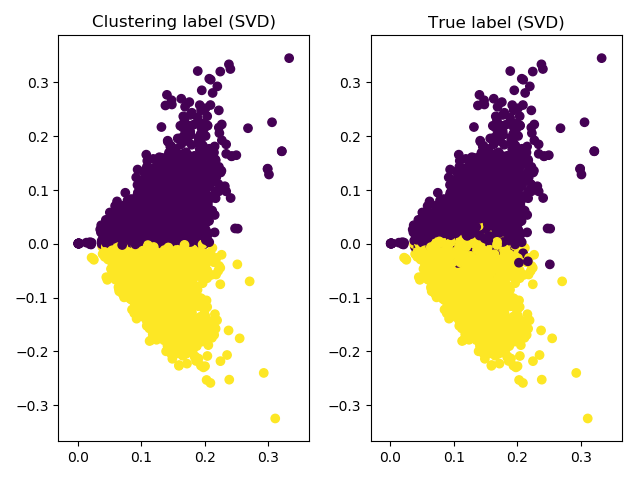
\includegraphics{Figure/Q7_SVD.png}}
\caption{Clustering result for SVD (r=2)} \label{Q7_SVD}
\end{figure}

\begin{figure}
\centering
\scalebox{0.4}{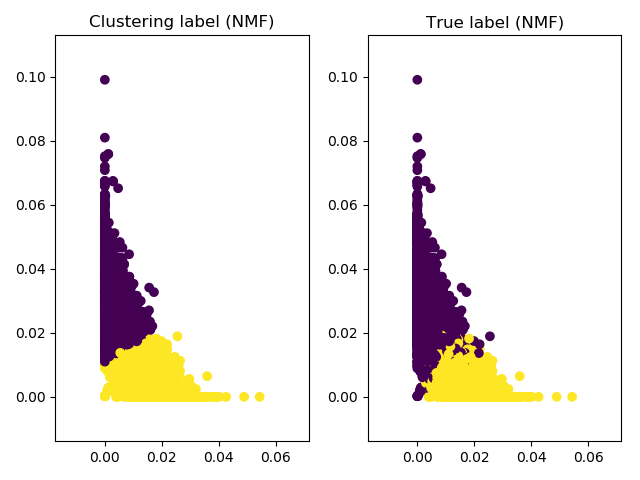
\includegraphics{Figure/Q7_NMF.png}}
\caption{Clustering result for NMF (r=2)} \label{Q7_NMF}
\end{figure}

\begin{table}[h]
\center
\caption{Confusion matrix for SVD (r=2)}
\scalebox{0.9}{
\begin{tabular}{r|c|c}
\hline
 & label = 0 & label = 1 \\\hline
label = 0 & 3656 & 247 \\\hline
label = 1 & 363 & 3616 \\\hline
\end{tabular}}
\label{tab:Q7_SVD_1}
\end{table}

\begin{table}[h]
\center
\caption{Performance for SVD (r=2)}
\scalebox{0.9}{
\begin{tabular}{r|c}
\hline
Homogeneity & 0.609 \\\hline
Completeness & 0.609 \\\hline
V measure & 0.609 \\\hline
Adjusted rand & 0.714 \\\hline
Adjusted mutual info & 0.609 \\\hline
\end{tabular}}
\label{tab:Q7_SVD_2}
\end{table}

\begin{table}[h]
\center
\caption{Confusion matrix for NMF (r=2)}
\scalebox{0.9}{
\begin{tabular}{r|c|c}
\hline
 & label = 0 & label = 1 \\\hline
label = 0 & 731 & 3172 \\\hline
label = 1 & 3943 & 36 \\\hline
\end{tabular}}
\label{tab:Q7_NMF_1}
\end{table}

\begin{table}[h]
\center
\caption{Performance for NMF (r=2)}
\scalebox{0.9}{
\begin{tabular}{r|c}
\hline
Homogeneity & 0.593 \\\hline
Completeness & 0.608 \\\hline
V measure & 0.600 \\\hline
Adjusted rand & 0.649 \\\hline
Adjusted mutual info & 0.593 \\\hline
\end{tabular}}
\label{tab:Q7_NMF_2}
\end{table}

From the distribution of the data points after SVD, we can observe that it is relatively harder to cluster them into 2 classes comparing to NMF, because most of the points are very close to each other and there is no clear boundary. In contrast, NMF is slightly better, showing a triangular distribution. These can be seen from \ref{tab:Q7_SVD_1} and \ref{tab:Q7_NMF_1}.

\subsection{Transformation Methods}

\textbf{Question 8:}

\begin{figure}
\centering
\scalebox{0.4}{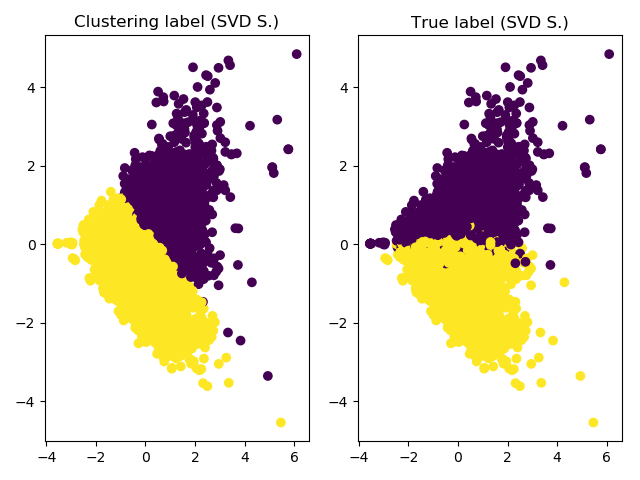
\includegraphics{Figure/Q8_SVD_scale.png}}
\caption{Normalized (scaling) clustering result for SVD (r=2)} \label{Q8_SVD_scale}
\end{figure}

\begin{figure}
\centering
\scalebox{0.4}{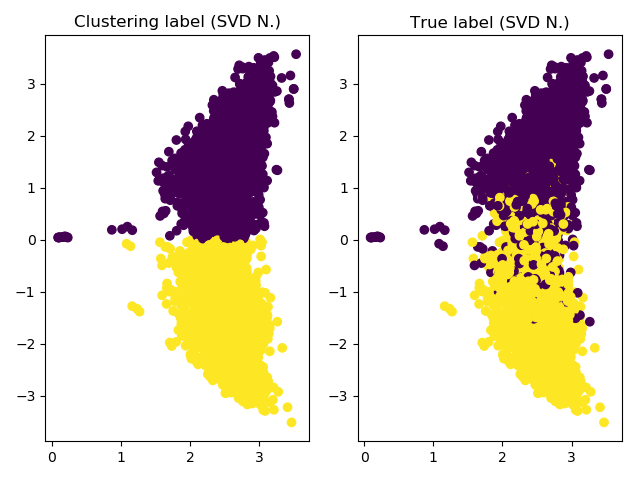
\includegraphics{Figure/Q8_SVD_nonlinear.png}}
\caption{Normalized (non-linear transformation) clustering result for SVD (r=2)} \label{Q8_SVD_nonlinear}
\end{figure}

\begin{figure}
\centering
\scalebox{0.4}{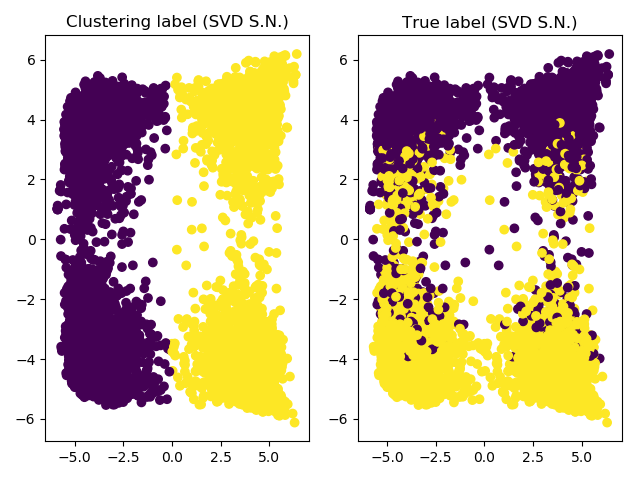
\includegraphics{Figure/Q8_SVD_scale_nonlinear.png}}
\caption{Normalized (scaling + non-linear transformation) clustering result for SVD (r=2)} \label{Q8_SVD_scale_nonlinear}
\end{figure}

\begin{figure}
\centering
\scalebox{0.4}{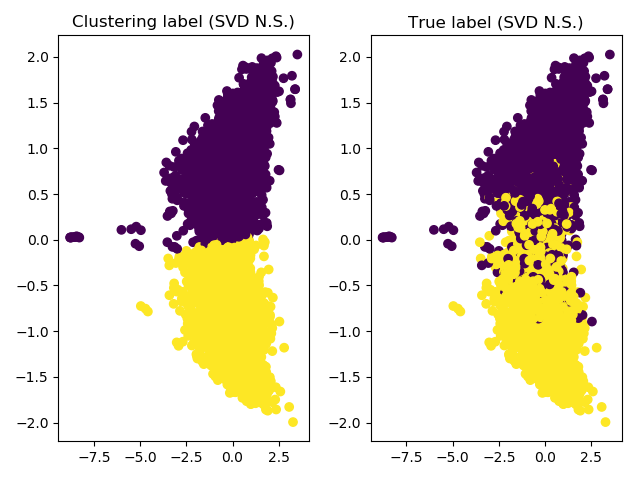
\includegraphics{Figure/Q8_SVD_nonlinear_scale.png}}
\caption{Normalized (non-linear transformation + scaling) clustering result for SVD (r=2)} \label{Q8_SVD_nonlinear_scale}
\end{figure}

\begin{figure}
\centering
\scalebox{0.4}{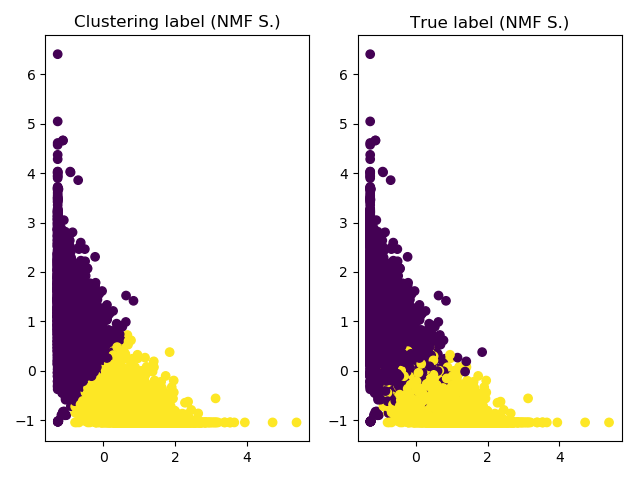
\includegraphics{Figure/Q8_NMF_scale.png}}
\caption{Normalized (scaling) clustering result for NMF (r=2)} \label{Q8_NMF_scale}
\end{figure}

\begin{figure}
\centering
\scalebox{0.4}{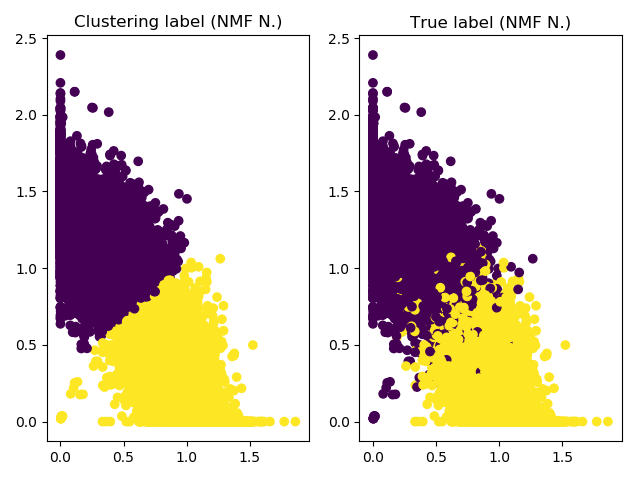
\includegraphics{Figure/Q8_NMF_nonlinear.png}}
\caption{Normalized (non-linear transformation) clustering result for NMF (r=2)} \label{Q8_NMF_nonlinear}
\end{figure}

\begin{figure}
\centering
\scalebox{0.4}{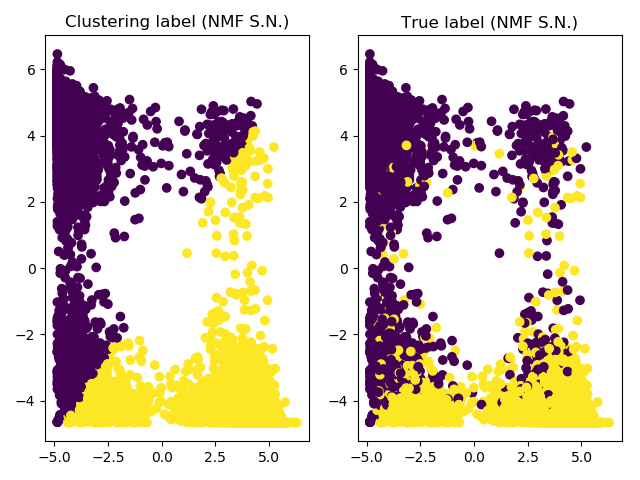
\includegraphics{Figure/Q8_NMF_scale_nonlinear.png}}
\caption{Normalized (scaling + non-linear transformation) clustering result for NMF (r=2)} \label{Q8_NMF_scale_nonlinear}
\end{figure}

\begin{figure}
\centering
\scalebox{0.4}{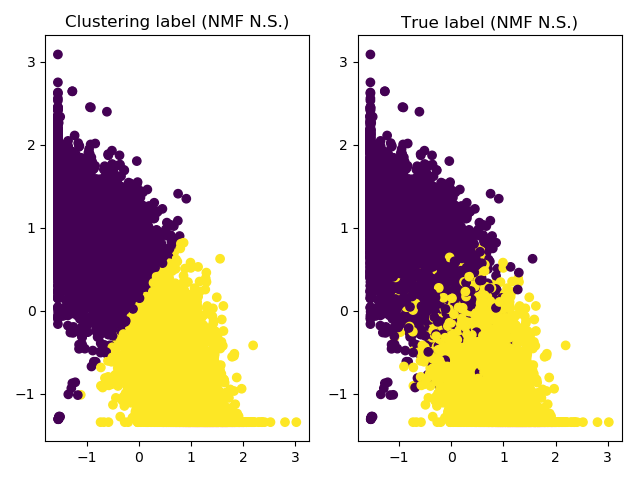
\includegraphics{Figure/Q8_NMF_nonlinear_scale.png}}
\caption{Normalized (non-linear transformation + scaling) clustering result for NMF (r=2)} \label{Q8_NMF_nonlinear_scale}
\end{figure}

In this question, we applied different normalization methods to see if they increase the clustering performance: 1) normalizing features such that each feature has unit variance; 2) applying a non-linear transformation to the data vectors; 3) combining both transformations (in different orders) on the data. 

\bigbreak

\textbf{Question 9:}

We found log transformation greatly improves the result. The reason is because the original data points are skewed with wide distribution, and taking the log of the features may restore symmetry to it. As we can see from the distribution of the observations after taking log, the points are mapped to a sector that is easier to cluster.

\textbf{Question 10:}

\begin{table}[h]
\center
\caption{Performance for SVD after normalization (scaling) (r=2)}
\scalebox{0.9}{
\begin{tabular}{r|c}
\hline
Homogeneity & 0.227 \\\hline
Completeness & 0.257 \\\hline
V measure & 0.241 \\\hline
Adjusted rand & 0.244 \\\hline
Adjusted mutual info & 0.227 \\\hline
\end{tabular}}
\label{tab:Q7_SVD_1}
\end{table}

\begin{table}[h]
\center
\caption{Performance for SVD after normalization (non-linear transformation) (r=2)}
\scalebox{0.9}{
\begin{tabular}{r|c}
\hline
Homogeneity & 0.609 \\\hline
Completeness & 0.609 \\\hline
V measure & 0.609 \\\hline
Adjusted rand & 0.716 \\\hline
Adjusted mutual info & 0.609 \\\hline
\end{tabular}}
\label{tab:Q7_SVD_2}
\end{table}

\begin{table}[h]
\center
\caption{Performance for SVD after normalization (scaling + non-linear transformation) (r=2)}
\scalebox{0.9}{
\begin{tabular}{r|c}
\hline
Homogeneity & 7.41e-05 \\\hline
Completeness & 7.43e-05 \\\hline
V measure & 7.42e-05 \\\hline
Adjusted rand & -1.32e-05 \\\hline
Adjusted mutual info & -1.74e-05 \\\hline
\end{tabular}}
\label{tab:Q7_SVD_3}
\end{table}

\begin{table}[h]
\center
\caption{Performance for SVD after normalization (non-linear transformation + scaling) (r=2)}
\scalebox{0.9}{
\begin{tabular}{r|c}
\hline
Homogeneity & 0.610 \\\hline
Completeness & 0.610 \\\hline
V measure & 0.610 \\\hline
Adjusted rand & 0.717 \\\hline
Adjusted mutual info & 0.609 \\\hline
\end{tabular}}
\label{tab:Q7_SVD_4}
\end{table}

\begin{table}[h]
\center
\caption{Performance for NMF after normalization (scaling) (r=2)}
\scalebox{0.9}{
\begin{tabular}{r|c}
\hline
Homogeneity & 0.682 \\\hline
Completeness & 0.685 \\\hline
V measure & 0.683 \\\hline
Adjusted rand & 0.773 \\\hline
Adjusted mutual info & 0.682 \\\hline
\end{tabular}}
\label{tab:Q7_NMF_1}
\end{table}

\begin{table}[h]
\center
\caption{Performance for NMF after normalization (non-linear transformation) (r=2)}
\scalebox{0.9}{
\begin{tabular}{r|c}
\hline
Homogeneity & 0.701 \\\hline
Completeness & 0.702 \\\hline
V measure & 0.702 \\\hline
Adjusted rand & 0.795 \\\hline
Adjusted mutual info & 0.701 \\\hline
\end{tabular}}
\label{tab:Q7_NMF_2}
\end{table}

\begin{table}[h]
\center
\caption{Performance for NMF after normalization (scaling + non-linear transformation) (r=2)}
\scalebox{0.9}{
\begin{tabular}{r|c}
\hline
Homogeneity & 0.695 \\\hline
Completeness & 0.695 \\\hline
V measure & 0.695 \\\hline
Adjusted rand & 0.792 \\\hline
Adjusted mutual info & 0.695 \\\hline
\end{tabular}}
\label{tab:Q7_NMF_3}
\end{table}

\begin{table}[h]
\center
\caption{Performance for NMF after normalization (non-linear transformation + scaling) (r=2)}
\scalebox{0.9}{
\begin{tabular}{r|c}
\hline
Homogeneity & 0.702 \\\hline
Completeness & 0.704 \\\hline
V measure & 0.703 \\\hline
Adjusted rand & 0.797 \\\hline
Adjusted mutual info & 0.702 \\\hline
\end{tabular}}
\label{tab:Q7_NMF_4}
\end{table}

All clustering measures are listed in \ref{tab:Q7_SVD_1}, \ref{tab:Q7_SVD_2}, \ref{tab:Q7_SVD_3}, \ref{tab:Q7_SVD_4}, \ref{tab:Q7_NMF_1}, \ref{tab:Q7_NMF_2}, \ref{tab:Q7_NMF_3}, \ref{tab:Q7_NMF_4}.

\section{Expand Dataset into 20 Categories}

\textbf{Question 11:}
The contingency matrix is as in the table \ref{tab:q11m}, and the five performance is as in the table \ref{tab:q11}
\begin{table}[h]
\center
\caption{The contingency matrix for 20 categories}
\begin{tabular}{c c c c c c c c c c c c c c c c c c c c}
 57 & 40 & 0 & 1 & 5 & 84 & 0 & 0 & 83 & 1 & 0 & 0 & 2 & 401 & 36 & 9 & 0 & 80 & 0 & 0  \\ 
 82 & 0 & 1 & 16 & 1 & 1 & 2 & 0 & 241 & 0 & 0 & 4 & 1 & 3 & 525 & 0 & 0 & 0 & 0 & 96  \\
 33 & 0 & 18 & 2 & 0 & 0 & 11 & 0 & 126 & 0 & 2 & 2 & 0 & 0 & 206 & 0 & 0 & 0 & 0 & 585  \\
 25 & 0 & 230 & 7 & 1 & 0 & 5 & 0 & 175 &  0 & 0 & 5 & 0 & 0 & 437 & 0 & 3 & 0 & 0 & 94  \\
 25 & 0 & 103 & 10 & 0 & 0 & 1 & 0 & 372 & 0 & 0 & 3 & 0 & 1 & 437 &  0  & 0 &  0 & 0 & 11  \\
 86 &  0 &  1 & 25 &  0 &  0 &  2 &  0& 143 &  3 &  0 &  4 &  0 &  1 &569 &  0 &  0 &  0 & 0 &154  \\
 5 &  0 & 70 &  3 & 27 &  0 &  7  & 0& 477  & 0 &  0  &12  & 5 &  0 &334 &  0 & 12 &  0 & 0  &23  \\
 18 &  0 &  0  & 7 &568 &  0 &  1 &  0 &210 &  0 &  0 &  5 &  3 &  0 &164 & 12 &  0 &  0 & 0 &  2  \\
 77 &  0 &  0 & 17& 682 &  0 &  1 &  0& 110 &  0 &  0 & 12 &  0 &  0 & 97 &  0  & 0  & 0 & 0 &  0  \\
 2  & 0 &  0 &  2 &  0 &  0  & 1  & 0 &312 &  0 &  0   &2  & 4 &  1& 171 &  0 &499 &  0&  0 &  0  \\
 2  & 0&   0 &  3  & 2 &  0  & 0  & 0& 110 &  0  & 0  &50  & 0  & 1  &83  & 0 &748  & 0 & 0  & 0  \\
 49 &  0 &  0 &  3 &  0 &  0 & 33 &  0 & 93 &543 &  0 &  0&  17   &3 &206 & 34 &  0 &  1 & 0 &  9  \\
 49  & 0&   8 & 35  &29  & 0 &  1  & 0 &242 &  1 & 13  & 7 &  0  & 0 &582 &  0 &  1  & 0 & 0 & 16  \\
 19   &0 &  0 & 18  & 0  & 1  & 4  &77 &251&   0 & 14 &  1 &  2 & 38 &560 &  3 &  0 &  0 & 0 &  2  \\
 21  & 0 &  0 &486  & 2   &0 &107  & 0& 140  & 0  & 0  & 0  & 1  & 9 &211  & 9  & 0  & 0 & 0  & 1  \\
 14  & 1 &  0  & 3  & 1 355 &  0 &  0 & 57  & 0 & 19 &  0 &  0 &439 &103 &  4 &  0 &  0 & 0 &  1  \\
 12  & 0  & 0 &  5  & 2  & 0  & 2 &  0& 118  & 4 &  0  & 5&  74&   3& 129 &556&   0  & 0&  0  & 0  \\
 5  & 0 &  0 &  0 &  0 &  2 &  0 &  0& 107 &  0  & 0 & 18  & 0 & 72 & 84 &238 &  0 &  0&  414 &  0  \\
 11 &  0 &  0&  12 &  1 &  2 &  1 &  0 &149  & 2 &  0 & 20 &  5 & 51& 161& 230 &  0& 130 & 0  & 0  \\
 14 & 71 &  0 &  0  & 2 & 93 &  4 &  2 & 81 &  0 &  0 & 13  & 1& 195&  85&  57 &  0 & 10 & 0  & 0  \\
\end{tabular}
\label{tab:q11m}
\end{table}



\begin{table}[h]
\center
\caption{5 measures for the 20 K-means clustering results}
\scalebox{0.9}{
\begin{tabular}{c|c}
\hline
Homogeneity & 0.3594 \\\hline
Completeness & 0.4511 \\\hline
V-measure & 0.4001 \\\hline
Adjusted Rand Index & 0.1366 \\\hline
Adjusted mutual info score & 0.3573\\\hline
\end{tabular}}
\label{tab:q11}
\end{table}


\textbf{Question 12:}
In the test, the best combination is using the scaling features first, and then non-linear transformation for transformation. And for dimension reduction, NMF is the best choice. For r, 2 is the best choice. The 5 measurement for such combination is as in the table\ref{tab:q12}

\begin{table}[h]
\center
\caption{5 measures for the 20 K-means clustering results after dimension reduction and transform}
\scalebox{0.9}{
\begin{tabular}{c|c}
\hline
Homogeneity & 0.2200 \\\hline
Completeness & 0.2241 \\\hline
V-measure & 0.2220 \\\hline
Adjusted Rand Index & 0.0730 \\\hline
Adjusted mutual info score & 0.2175\\\hline
\end{tabular}}
\label{tab:q12}
\end{table}

\end{document}
